\documentclass[11pt]{article}
\usepackage[margin=2.5cm]{geometry}
\usepackage[utf8]{inputenc}
\usepackage[spanish]{babel}
\usepackage{graphicx}
\usepackage{amsmath}
\usepackage{amssymb}
\usepackage{booktabs}
\usepackage{hyperref}
\usepackage{float}

\title{Gemelo digital del beamline: un hurdle model físicamente informado}
\author{Taller MIT--UNAL, Medellín}
\date{}

\begin{document}
\maketitle

\section{La cantidad que modelamos}

Elegimos modelar la \textbf{transmisión}: el número de los 500 iones $^{28}$Si$^+$ que
llegan a la caja del detector, para un vector de 8 voltajes
$(V_3, V_6, V_9, V_{10}, V_{11}, V_{12}, V_{15}, V_{18})$. Es la cantidad más directa
para las dos tareas de control que pide el reto (maximizar transmisión, y alcanzar una
consigna de transmisión), y es la que ya veníamos generando con
\texttt{optimizer.py} (Optuna + SIMION real), así que aprovechamos ese historial de datos
en vez de reconfigurar la grabación del banco de trabajo para otra cantidad (velocidad,
dispersión espacial, etc.).

\section{Recolección de datos}

\texttt{optimizer.py} ya había generado \textbf{824 corridas reales de SIMION} antes de
empezar este proyecto (búsqueda bayesiana con Optuna). De esas, 330 fallaron con un error
de subproceso. Investigamos la causa: no es una región de voltaje físicamente prohibida
—repetir a mano esos mismos voltajes corrió sin problema— sino un patrón de fallas en
ráfagas concentradas en el tiempo, consistente con el proyecto viviendo dentro de una
carpeta sincronizada con OneDrive (la sincronización compite por el acceso al archivo
\texttt{electrode\_.PA0}, de 289\,MB, que se reescribe en cada evaluación). Recomendamos
excluir la carpeta de la sincronización; después de hacerlo, la tasa de error cayó a
prácticamente cero.

Quedaron \textbf{494 evaluaciones reales válidas} (130 con señal, 364 en cero). El
presupuesto de entrenamiento asignado es de \textbf{100 evaluaciones}. En vez de gastar
presupuesto nuevo, elegimos \textbf{100 de esos 494 puntos ya existentes} mediante
\emph{farthest-point sampling} (muestreo de máxima distancia mínima), aplicado por
separado sobre el subconjunto con señal y el subconjunto en cero (45 y 55 puntos
respectivamente), para garantizar que el pico de transmisión quedara bien representado
aunque sea la minoría de los datos. Los 394 puntos reales restantes, nunca usados para
entrenar, quedan como un conjunto de validación gratuito y mucho más grande que cualquier
holdout sintético (Figura~\ref{fig:cobertura}).

\begin{figure}[H]
  \centering
  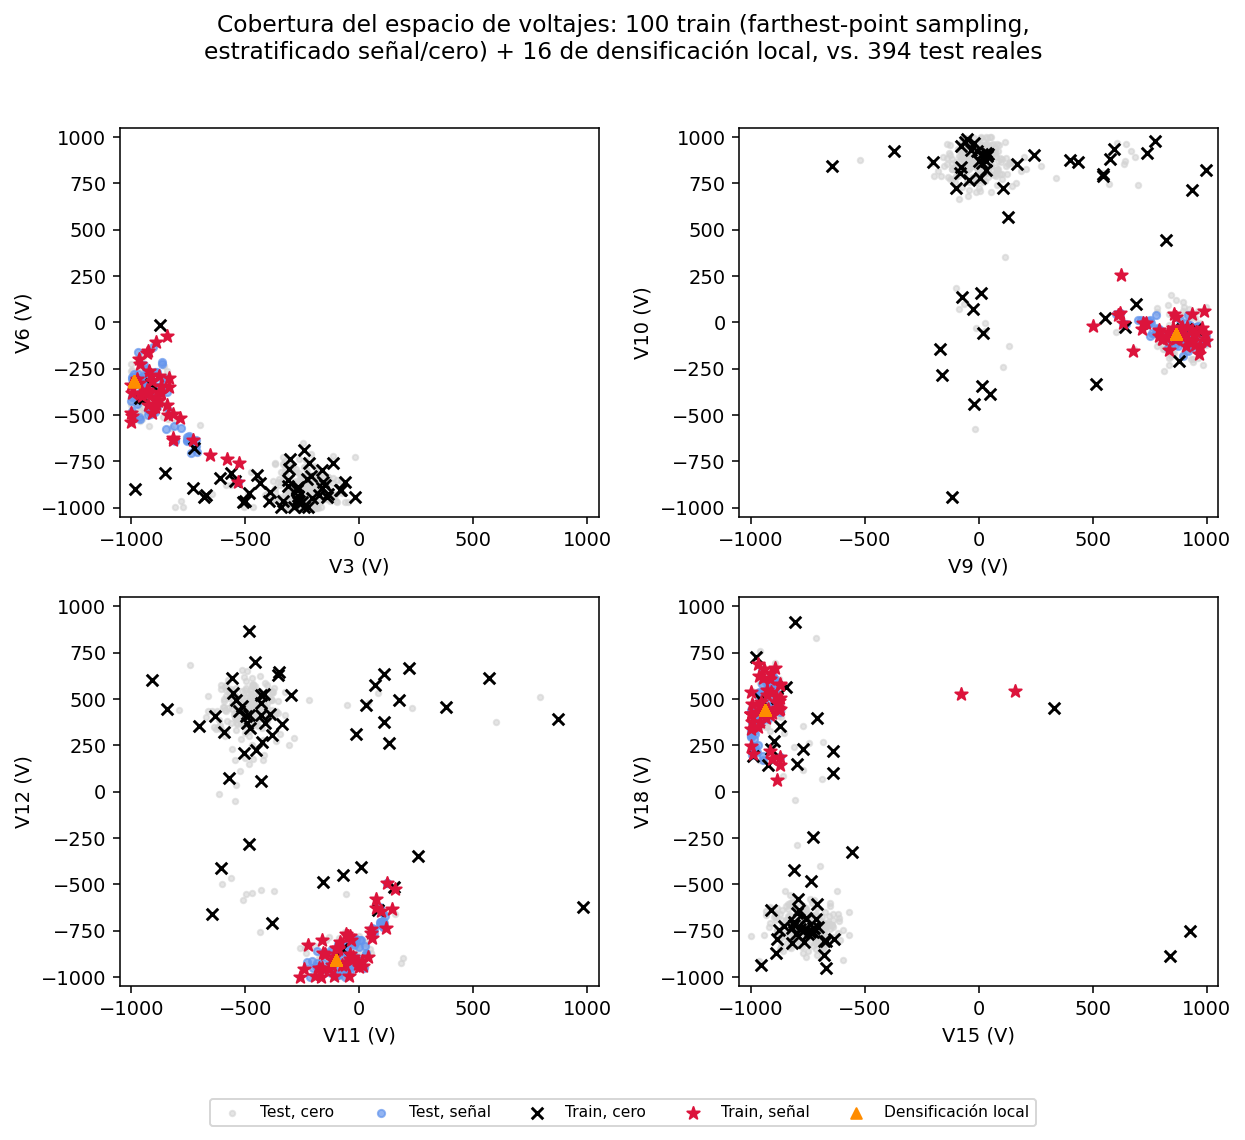
\includegraphics[width=0.95\textwidth]{figures/fig1_cobertura.png}
  \caption{Cobertura del espacio de voltajes en cuatro proyecciones 2D. Los 100 puntos de
  entrenamiento (cruces y estrellas) se distribuyen por todo el rango explorado por
  Optuna, no solo cerca del pico. Los triángulos naranjas son los 16 puntos de
  densificación local (Sección~\ref{sec:reflexion}).}
  \label{fig:cobertura}
\end{figure}

Adicionalmente, densificamos localmente con 16 puntos reales alrededor del mejor voltaje
conocido (los mismos usados para el chequeo de gradiente, Sección~\ref{sec:control}),
cada uno promediado sobre 5 corridas reales de SIMION por el ruido intrínseco que
describimos en la Sección~\ref{sec:reflexion}. En total: \textbf{100 (presupuesto
declarado) + 16 (densificación local) = 116 puntos de entrenamiento}, usando 180
llamadas reales a SIMION en total (100 + 16$\times$5).

\section{El modelo}

\subsection{Arquitectura: hurdle model}

La transmisión tiene una \textbf{zona muerta} grande (364/494 = 74\,\% de los puntos
válidos dan cero) y una región de señal angosta. Un solo GP tratando de ajustar ambos
regímenes a la vez predice cerca de cero en todas partes y falla exactamente donde más
importa. Por eso separamos el problema en dos etapas (\emph{hurdle model}):

\begin{itemize}
  \item \textbf{Etapa A — clasificador}: un \texttt{GaussianProcessClassifier} (kernel
  RBF con un length-scale por dimensión, ARD) entrenado con los 116 puntos completos
  (señal y cero), predice $P(\text{señal}\mid V)$.
  \item \textbf{Etapa B — regresor de magnitud}: un GP (kernel
  $\text{ConstantKernel}\times\text{Mat\'ern}_{\nu=1.5}\text{(ARD)} +
  \text{WhiteKernel}$, con \texttt{log1p} en la salida y \texttt{StandardScaler} en
  entradas y salida) entrenado \textbf{solo} con los puntos de señal, para que la
  campana no compita contra los vecinos en cero. Elegimos Mat\'ern $\nu=1.5$ sobre RBF
  comparando en el test real de 394 puntos: el pico de transmisión es angosto y la
  respuesta no es infinitamente suave, que es justo lo que RBF asume ($R^2$ informativa:
  0.237 con Mat\'ern 1.5, 0.232 con Mat\'ern 2.5, 0.203 con RBF;
  \texttt{kernel\_experiment.py}).
\end{itemize}

\subsection{Feature física: ley $V^2$ de la lente Einzel}

Una lente Einzel enfoca el haz sin importar el signo de su voltaje central —la potencia
de enfoque escala como $(V_{\text{lente}}/V_{\text{haz}})^2$ (fórmula de lente delgada
electrostática)—, así que agregamos $V_3^2$ y $V_6^2$ como entradas adicionales (10
dimensiones en total). Probamos también la hipótesis de que el curvador cuadrupolar
fuera antisimétrico ($V_9=-V_{10}$, $V_{11}=-V_{12}$, como asumimos al prototipar con un
simulador sintético) y la \textbf{rechazamos}: las correlaciones reales entre esas sumas
y la transmisión son débiles y de signo contrario al esperado (-0.16 a 0.14), y tiene
sentido físico —un curvador que dobla el haz 90$^\circ$ necesita una componente de dipolo
neto, no puede ser puramente antisimétrico. No la impusimos; dejamos que el kernel ARD
aprenda esa correlación directamente.

\subsection{Combinando las dos etapas}

Modelamos $T = Z\cdot M$ con $Z\sim\text{Bernoulli}(p)$ y $M$ la magnitud (media
$\mu_B$, varianza $\sigma_B^2$). Por ley de varianza total:
\begin{equation}
  \mathbb{E}[T] = p\,\mu_B, \qquad
  \text{Var}[T] = p(1-p)\,\mu_B^2 + p\,\sigma_B^2 .
\end{equation}
El primer término crece cuando el clasificador no sabe si hay señal; el segundo, cuando
el regresor no sabe cuánta. Ambas salidas se recortan a $[0,500]$ (criterio de
admisibilidad).

\section{Resultados}

\subsection{Predicho vs.\ real en la región informativa}

Validamos contra los 394 puntos de test reales, nunca usados en entrenamiento. En la
región informativa (85 de esos puntos con señal): $R^2=0.237$, MAE $=9.0$ iones
(Figura~\ref{fig:predicho}). El clasificador tiene \emph{accuracy}$=0.845$,
\emph{precision}$=0.582$ y, sobre todo, \textbf{recall}$=1.000$: nunca descarta un punto
que en realidad sí tiene señal, aunque a cambio marca de más algunos puntos en cero como
posible señal — el error que preferimos, dado que el costo de perderse la región buena es
mucho mayor.

\begin{figure}[H]
  \centering
  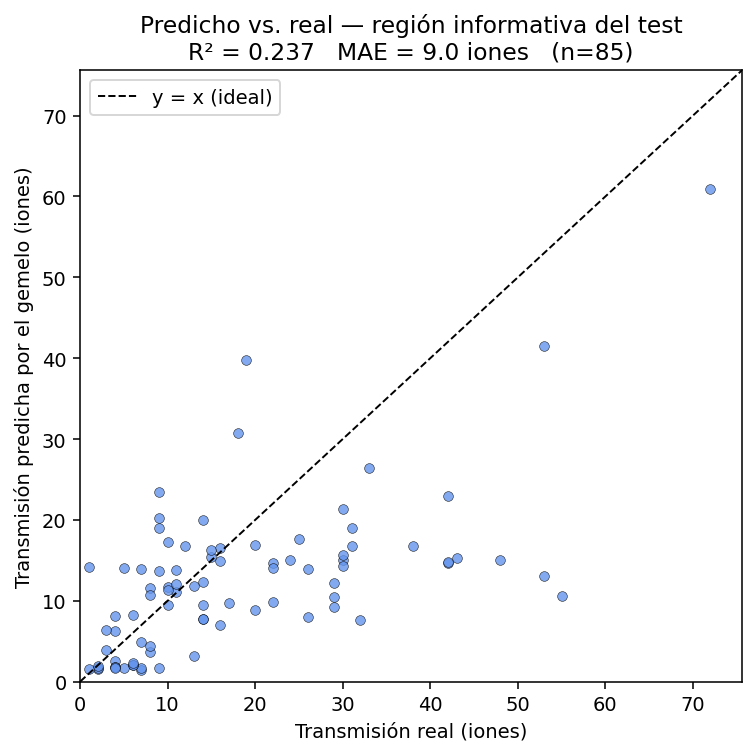
\includegraphics[width=0.62\textwidth]{figures/fig2_predicho_vs_real.png}
  \caption{Transmisión predicha vs.\ real, solo en los 85 puntos de test con señal.}
  \label{fig:predicho}
\end{figure}

\subsection{Honestidad de la incertidumbre}

La desviación estándar combinada (Figura~\ref{fig:honestidad}) es más alta justo donde
el clasificador está indeciso ($P(\text{señal})\in[0.4,0.6]$: std$\approx 11$ iones) y más
baja donde está seguro (std$\approx 6$--7 iones cerca de 0 o 1) — el comportamiento que
exige el criterio de honestidad/extrapolación.

\begin{figure}[H]
  \centering
  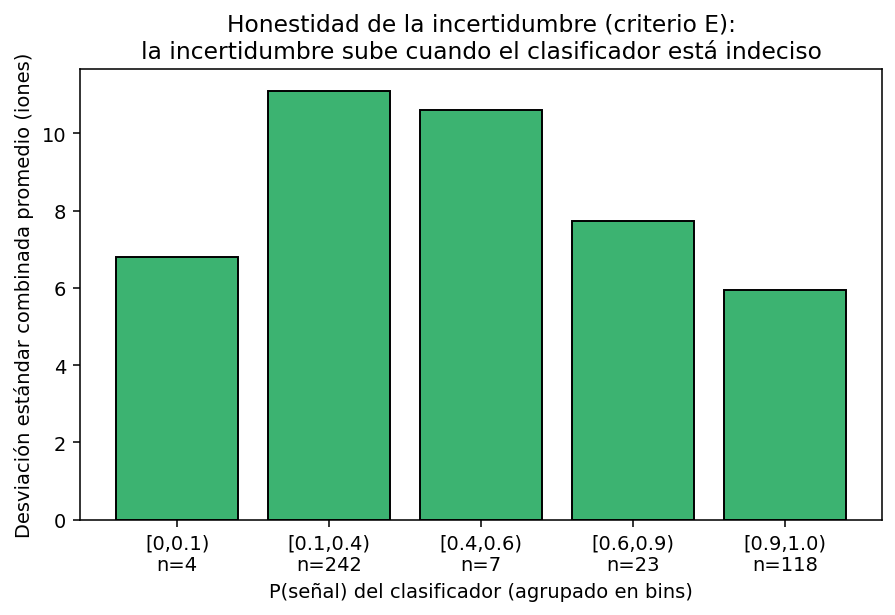
\includegraphics[width=0.62\textwidth]{figures/fig3_honestidad_incertidumbre.png}
  \caption{La incertidumbre combinada crece cuando el clasificador está indeciso.}
  \label{fig:honestidad}
\end{figure}

\section{Control}
\label{sec:control}

\subsection{El problema: optimizar libremente sobre el gemelo es peligroso}

La primera versión de la tarea de dirección optimizó \texttt{predict\_combined} sin
restricciones sobre todo $\pm1000\,$V. Predijo 34.9 iones; verificado con SIMION real dio
\textbf{0 iones}. Penalizar la incertidumbre en el objetivo (\emph{lower confidence
bound}) tampoco lo arregló: el modelo estaba \emph{seguro} (std bajo) justo donde se
equivocaba. Diagnóstico: con solo 45 puntos de señal en 8D, el pico real es más angosto de
lo que el GP puede resolver.

\subsection{La solución: radio de confianza calibrado con SIMION real}

En vez de optimizar sobre todo el espacio, restringimos la búsqueda a una vecindad
alrededor del mejor voltaje real conocido (72 iones), y calibramos el radio corriendo
SIMION real a varios valores:

\begin{center}
\begin{tabular}{lcccccc}
\toprule
Radio (V) & 150 & 40 & 20 & 15 & 10 & 5 \\
\midrule
Transmisión real & 1 & 0 & 18 & 31 & 29 & 39--52 \\
\bottomrule
\end{tabular}
\end{center}

Se fijó \textbf{radio $=5\,$V para la dirección} (el mejor resultado real).

Para la consigna inversa aplicamos el mismo principio pero con una mejora: la primera
versión anclaba también en el pico (72 iones) y dejaba que el gemelo modelara la ladera
descendente de la campana hasta el objetivo (35 iones) — justo donde la campana es más
empinada — y el resultado real quedó en 48.8 iones (error de 13.8). La versión final
\textbf{ancla la vecindad en el punto real cuya transmisión observada está más cerca del
objetivo} (33 iones) y deja que el gemelo solo haga la interpolación fina local, con el
mismo radio de 5\,V (calibrado de nuevo: radio 10\,V dio error real de 7.0 iones; radio
5\,V, de 1.8). Es la misma división del trabajo que en la dirección: el dato real aporta
la región, el gemelo el ajuste fino.

\subsection{Resultado final verificado}

Cada número reportado es el promedio de 5 corridas reales de SIMION (ver
Sección~\ref{sec:reflexion} sobre por qué es necesario promediar).

\begin{center}
\small
\begin{tabular}{lccp{4.2cm}}
\toprule
Tarea & Predicho & Real (SIMION, prom.\ 5) & Resultado \\
\midrule
Dirección (max.) & 63.3 & $55.2\pm6.4$ & $C=0.767$ (77\,\% del óptimo, 72 iones) \\
Consigna (obj.=35) & 29.9 & $36.8\pm5.0$ & error $=1.8$ iones ($<$ ruido de la máquina) \\
\bottomrule
\end{tabular}
\end{center}

\begin{figure}[H]
  \centering
  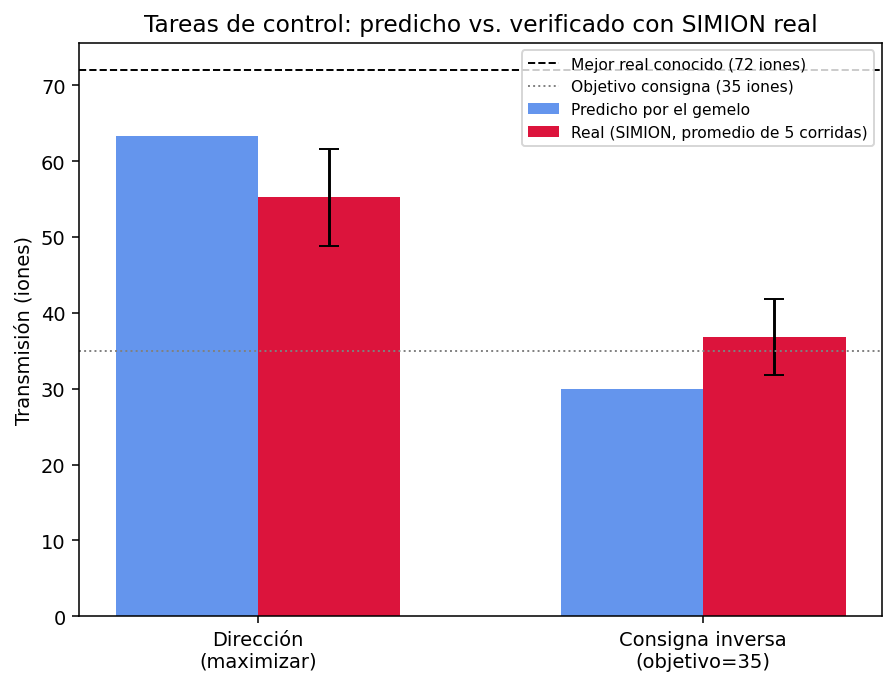
\includegraphics[width=0.62\textwidth]{figures/fig4_control.png}
  \caption{Resultados de control: predicho por el gemelo vs.\ verificado con SIMION real.}
  \label{fig:control}
\end{figure}

\subsection{Diferenciabilidad (criterio D)}

Comparamos el gradiente del gemelo contra diferencias finitas de SIMION real
($\varepsilon=1\,$V) en el punto ancla (Figura~\ref{fig:gradiente}). Antes de la
densificación local, la similitud coseno entre ambos gradientes era $-0.612$
—¡apuntaban casi en dirección opuesta! Después de densificar con los 16 puntos reales
locales, subió a $-0.049$: ya no contradice la realidad, pero tampoco concuerda bien
todavía.

\begin{figure}[H]
  \centering
  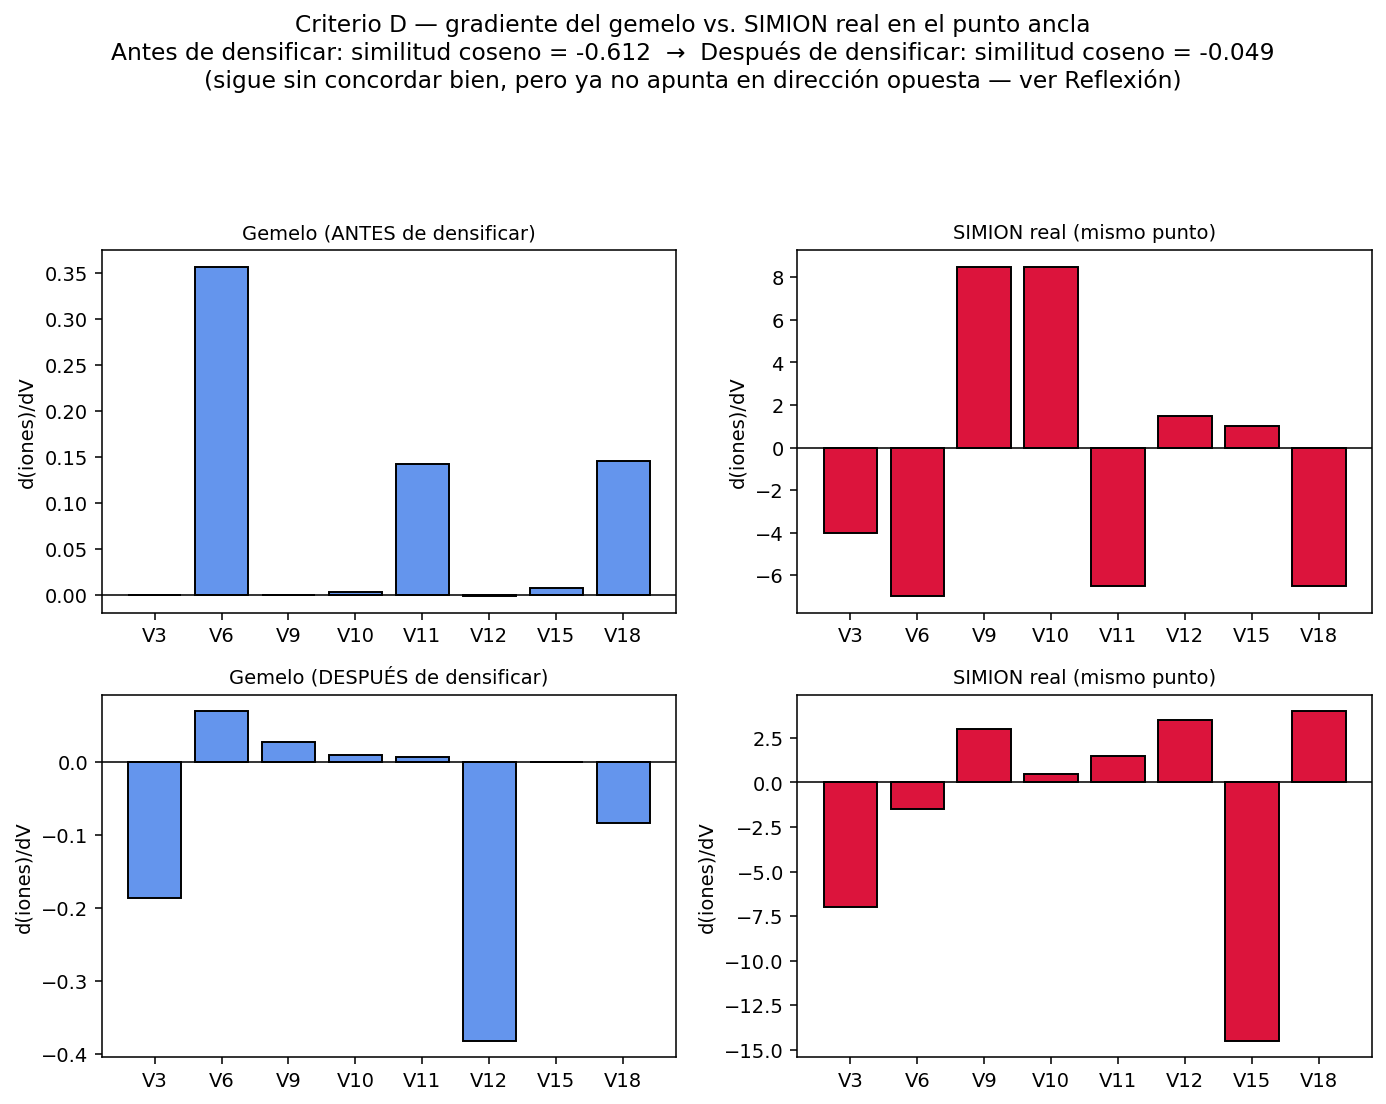
\includegraphics[width=0.85\textwidth]{figures/fig5_gradiente.png}
  \caption{Gradiente del gemelo vs.\ SIMION real, antes y después de la densificación
  local.}
  \label{fig:gradiente}
\end{figure}

\subsubsection{El paso $\varepsilon=1\,$V era el problema, no (solo) el gemelo}

Analizando el ruido de SIMION (Sección~\ref{sec:reflexion}) encontramos que la
comparación anterior no podía funcionar: cada conteo, aun promediado sobre 5 corridas,
conserva una incertidumbre de $\approx 3$--$4$ iones (std $\approx 6$--$10$ entre
corridas individuales). Una diferencia centrada hereda entonces un ruido de
$\sim \sqrt{2}\cdot 4/(2\varepsilon) \approx 2.8/\varepsilon$ iones/V. Con
$\varepsilon=1\,$V eso es $\pm 2.8$ iones/V — mayor que el gradiente verdadero
($|\partial T/\partial V| \lesssim 1$ ion/V en el ancla): \textbf{el ``gradiente real''
de referencia era ruido puro}, y la similitud coseno medía azar, no al gemelo.

Repetimos el chequeo con pasos más grandes (16 puntos $\times$ 5 corridas reales por
cada $\varepsilon$; son corridas de \emph{verificación}, que según el enunciado no
cuentan contra el presupuesto de entrenamiento):

\begin{center}
\begin{tabular}{lccc}
\toprule
Paso $\varepsilon$ & 1\,V & 5\,V & 10\,V \\
\midrule
Similitud coseno & $-0.241$ & $\mathbf{+0.307}$ & $+0.059$ \\
\bottomrule
\end{tabular}
\end{center}

Con $\varepsilon=5\,$V la relación señal/ruido mejora $\times 5$ y la similitud pasa a
$+0.307$: el gradiente del gemelo \textbf{sí apunta en la dirección correcta} cuando se
mide a la escala que el ruido de la máquina permite (Figura~\ref{fig:gradiente_eps}).
Con $\varepsilon=10\,$V vuelve a caer: el pico real tiene un ancho del orden de
10--20\,V (Sección~\ref{sec:control}), así que la secante a $\pm 10\,$V ya se sale de
la campana — sesgo de curvatura. Existe una ventana intermedia
($\varepsilon \approx 5\,$V) entre el ruido y el sesgo, y es ahí donde el chequeo de
diferenciabilidad es informativo.

Como chequeo adicional, reentrenar el gemelo agregando las 16 sondas de
$\varepsilon=10\,$V (datos reales ya pagados) sube la similitud a $+0.469$ contra el
gradiente de $\varepsilon=5\,$V como conjunto \emph{held-out}. No incorporamos ese
reentrenamiento al modelo entregado —esas sondas están apiñadas alrededor del ancla y
degradan el ajuste \emph{global} ($R^2$ informativa cae de $0.237$ a $-0.07$ si se
agregan las 32 al entrenamiento; \texttt{retrain\_experiment.py}): mejoran el gradiente
local a costa del resto del espacio— pero confirma que el acuerdo del gradiente sigue
mejorando con datos locales \emph{bien balanceados}.
(Código: \texttt{gradient\_eps\_study.py} y \texttt{gradient\_retrain\_check.py},
con los datos reales congelados en \texttt{gradient\_eps\_study\_cache.npz}.)

\begin{figure}[H]
  \centering
  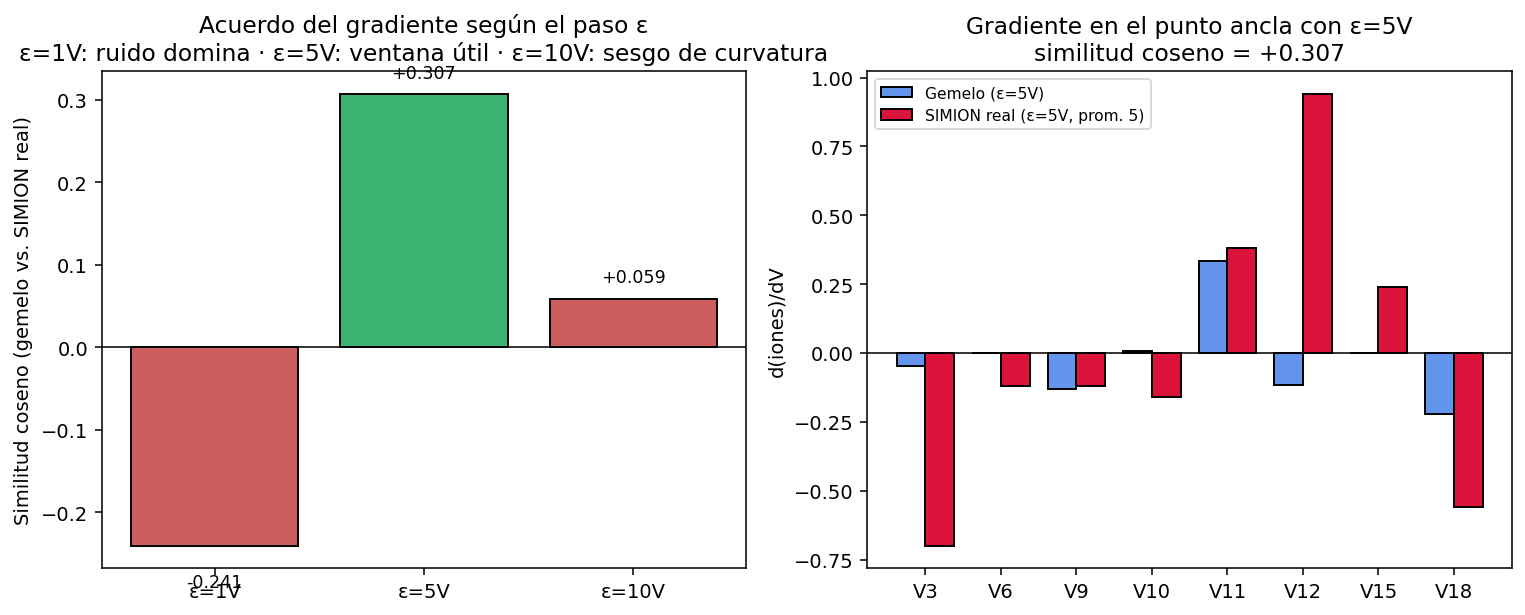
\includegraphics[width=0.95\textwidth]{figures/fig6_gradiente_eps.png}
  \caption{Izquierda: acuerdo del gradiente según el paso $\varepsilon$ — ruido a
  $\varepsilon$ pequeño, sesgo de curvatura a $\varepsilon$ grande, ventana útil en
  $\varepsilon=5$\,V. Derecha: gradiente del gemelo vs.\ SIMION real con
  $\varepsilon=5$\,V, componente por componente.}
  \label{fig:gradiente_eps}
\end{figure}

\section{Metodología: por qué este camino y no otro}

Consideramos y probamos varias alternativas antes de asentarnos en esta arquitectura:

\begin{itemize}
  \item \textbf{PINNs}: descartadas — no hay una PDE simple que relacionar 8 voltajes con
  el conteo final (esa relación ES la integración completa de trayectorias que SIMION ya
  resuelve); hubiéramos terminado reimplementando SIMION en una red neuronal.
  \item \textbf{Hamiltonian GNN}: descartada — necesita datos de trayectoria que no
  grabamos (el vuelo corre con \texttt{retain-trajectories=0}) y no hay una estructura de
  grafo natural en 8 voltajes escalares.
  \item \textbf{Regresión simbólica}: riesgosa como modelo principal en 8D con zona
  muerta; la dejamos como posible capa de interpretabilidad futura sobre el GP ya
  entrenado, no como apuesta central.
  \item \textbf{GP simple (sin hurdle, sin features físicas)}: nuestra línea base.
  $R^2$ en región informativa $=-0.338$ (peor que predecir el promedio). Justificó todo
  lo que sigue.
  \item \textbf{Hurdle model + features físicas}: subió el $R^2$ a $0.203$ (con
  densificación). Cambiar el kernel del regresor de RBF a Mat\'ern $\nu=1.5$ lo llevó a
  $\mathbf{0.237}$. Mejora real, aunque modesta — la escasez de datos de señal (45--61
  puntos) sigue siendo el techo.
  \item \textbf{Densificar el entrenamiento con las 32 sondas de gradiente extra}:
  probado y \textbf{descartado} — puntos tan apiñados alrededor del ancla desequilibran
  el GP y el $R^2$ global cae a $-0.07$ (\texttt{retrain\_experiment.py}). La
  densificación local útil fue la primera (16 puntos), no acumular más en el mismo sitio.
  \item \textbf{Optimización de control sin restricción}: falló catastróficamente (0
  iones reales). El radio de confianza, calibrado empíricamente con SIMION real, fue
  necesario para un resultado utilizable.
\end{itemize}

\section{Reflexión}
\label{sec:reflexion}

\subsection{Hasta dónde confiamos en el gemelo}

Confiamos en el gemelo \textbf{dentro de vecindades de $\pm5\,$V de puntos reales
conocidos}: ahí, con el radio de confianza calibrado, recomienda voltajes que de verdad
funcionan (77\,\% del óptimo real en la dirección; error de 1.8 iones —menor que el
ruido de la máquina— en la consigna inversa). \textbf{No confiamos}
en él para optimización libre sobre todo el rango $\pm1000\,$V: ya demostramos que puede
estar seguro y equivocado al mismo tiempo, y ni penalizar la incertidumbre lo arregla. El
$R^2$ de $0.237$ en la región informativa, aunque mejor que la línea base, sigue
indicando que el modelo no ha terminado de aprender la forma fina del pico — con 45--61
puntos de señal en 8 dimensiones, es un límite esperable, no una sorpresa.

\subsection{Un descubrimiento que cambió el proyecto: SIMION es ruidoso}

A mitad de la iteración de control encontramos que \textbf{el mismo punto exacto de
voltajes da resultados distintos en SIMION en corridas separadas} (74, 60 y 63 iones en
tres corridas del mismo punto; el archivo \texttt{SimpleSetUp.fly2} confirma por qué:
la energía cinética (\texttt{gaussian\_distribution}) y la dirección
(\texttt{cone\_direction\_distribution}) de los 500 iones se muestrean al azar en cada
vuelo). Revisamos el manual de SIMION 8.1: existe \texttt{simion.seed()}, pero solo se
puede invocar desde un programa Lua adjunto al workbench, no desde \texttt{--nogui fly}
ni desde el \texttt{.fly2}. En vez de modificar el workbench compartido, optamos por
\textbf{promediar 5 corridas reales} para cualquier número que reportamos como
verificación — esto también explica en parte por qué el $R^2$ y el gradiente eran tan
inestables entre intentos tempranos: no era solo falta de datos, era ruido de medición
real que no habíamos cuantificado.

\subsection{Qué mejoraría con más presupuesto}

Con más evaluaciones reales cerca del pico (más allá de las 16 de densificación),
esperaríamos que el $R^2$ de la región informativa siga subiendo y que el gradiente del
gemelo termine de alinearse con la realidad — la mejora que ya vimos al pasar de 45 a 61
puntos de señal ($R^2$ de $0.056$ a $0.203$, y a $0.237$ con el kernel final) sugiere que
el techo aún no se alcanzó. Eso sí, los puntos nuevos deben repartirse (por ejemplo con
muestreo activo guiado por incertidumbre), no acumularse en el mismo sitio: ya vimos que
32 sondas apiñadas degradan el ajuste global. También
valdría la pena investigar más a fondo la otra fuente de fallas de \texttt{optimizer.py}
(211 de 330 errores no se explican por la interferencia de OneDrive que sí confirmamos).

\end{document}
